\input ../SlidePreamble
\input ../preamble


\begin{document}

{\Huge
  \centerline{\bf TTIC 31230,  Fundamentals of Deep Learning, Winter 2019}
  \vfill
  \centerline{David McAllester}
  \vfill
  \centerline{\bf Pretraining}


\slide{Supervised Pretraining}

\vfill
We train a general purpose model and then fine tune that model on a different task.

\vfill
This has been standard practice with Imagenet models since 2013.

\vfill
General Learning Algorithms vs. Learning General Knowledge.

\slide{Example: R-CNN, Girshick et al., Nov. 2013}

\centerline{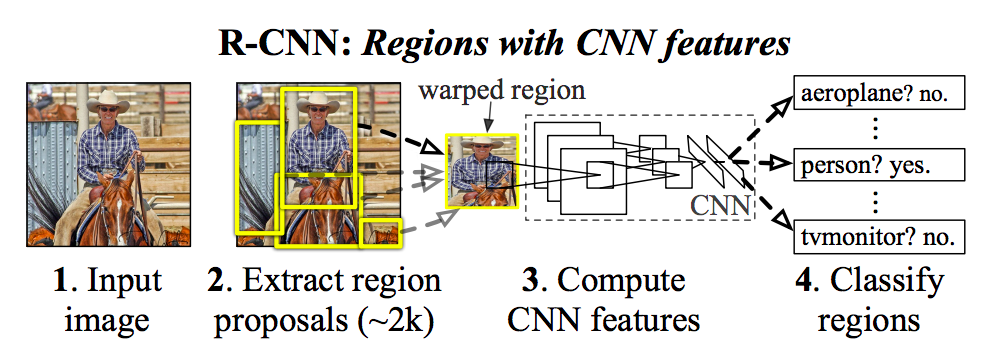
\includegraphics[width=10.0 in]{../images/R-CNN}}

Note that Alexnet appeared on the scene at the ImageNet evaluation (ILSVRC2012) Oct. 2012.

\slide{Instagram Pretraining, Mahajan et al., May 2018}

In our experiments, we train standard convolutional network architectures to
predict hashtags on up to 3.5 billion public Instagram images.

\vfill
To make training at this scale practical, we adopt a distributed synchronous implementation of
stochastic gradient descent with large (8k image) minibatches, following Goyal et al. 2017.

\slide{Instagram Pretraining}

\centerline{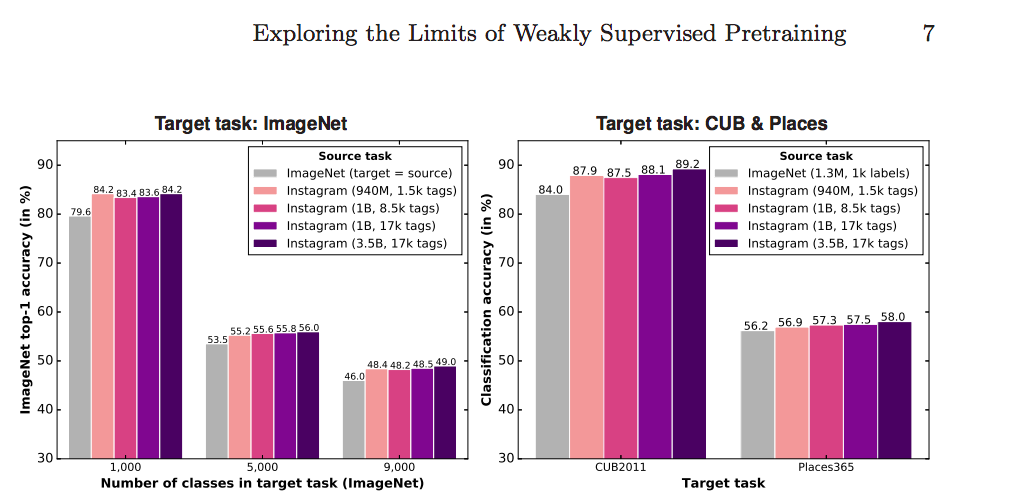
\includegraphics[width=10.0 in]{../images/InstagramPre}}

\slide{Rethinking ImageNet Pretraining, He et al., Nov. 2018}

We report competitive results on object detection and instance segmentation on the COCO dataset using standard
models trained from {\bf random initialization}.


\slide{Rethinking ImageNet Pretraining, He et al., Nov. 2018}

\centerline{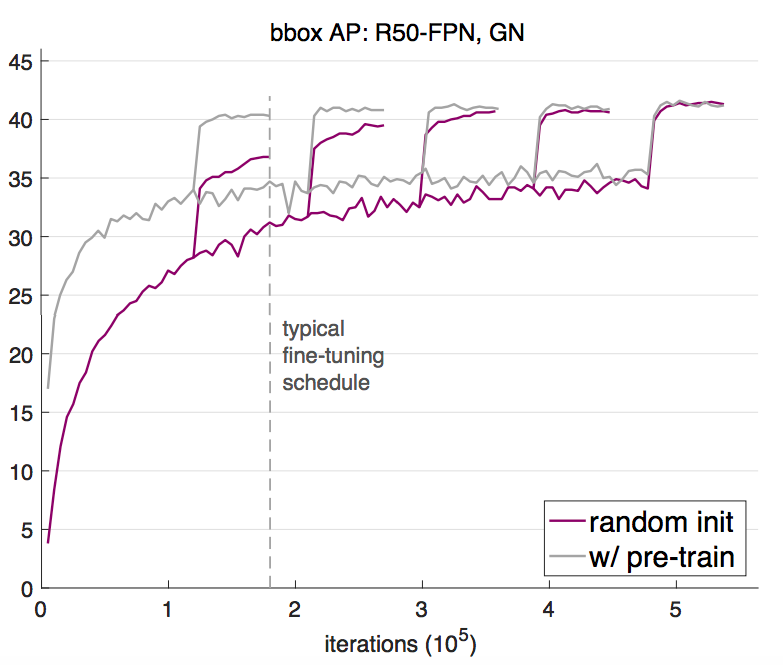
\includegraphics[width=6.0 in]{../images/RethinkingPre}}

\slide{Self-Supervised Pretraining}

We find some naturally occuring source of $(x,y)$ pairs and then treat it as a supervised learning problem.

\vfill
We then initialize learning models the weights derived from pretraining.

\vfill
We will consider inpainting and colorization.

\slidetwo{Feature Learning by Inpainting}{Pathak et al., April 2016}

$${\color{red} \Phi^* = \argmin_{\Phi}\; E_{(x,y) \sim \pop}\;||y - \hat{y}_\Phi(x)||^2 + \lambda \mathrm{Discr}(y,\hat{y}_\Phi(x))}$$

\centerline{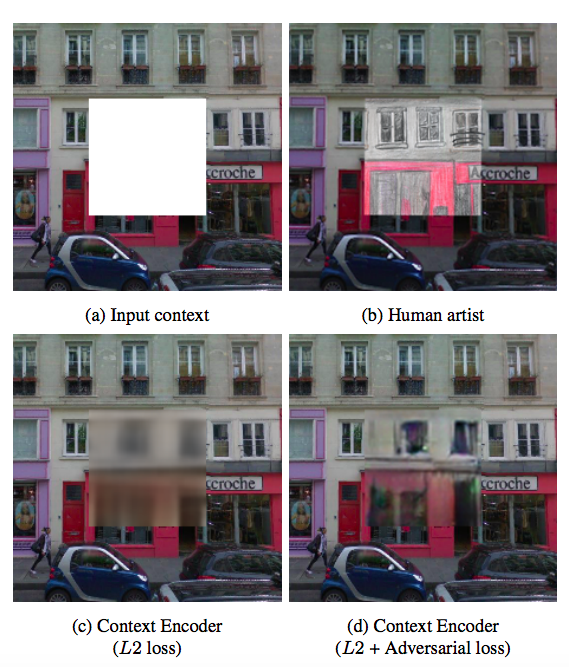
\includegraphics[width = 3in]{../images/LearnRepInpa}}

\slidetwoplain{Feature Learning by Inpainting}{Pathak et al., April 2016}

\centerline{\includegraphics[width = 9in]{../images/LearnRepINpb}}
\centerline{Alexnet, Trained on Imagenet, Evaluated on PASCAL}
\centerline{Image Count: {\color{red} Instagram 3.5G, ImageNet 14M, Pascal 5.7k}}

\slidetwo{Learning Representations for Colorization}{Larsson et al., March 2016}

{\color{red} $$\Phi^* = \argmin_\Phi \;E_{x,y \sim \pop}\; ||y - \hat{y}_\Phi(x)||^2$$}

\vfill
\centerline{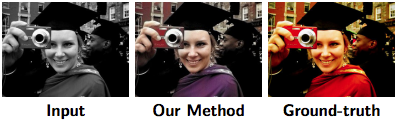
\includegraphics[width = 6in]{../images/colorizationGreg2}}

\slidetwo{Learning Representations for Colorization}{Larsson et al., March 2016}

\centerline{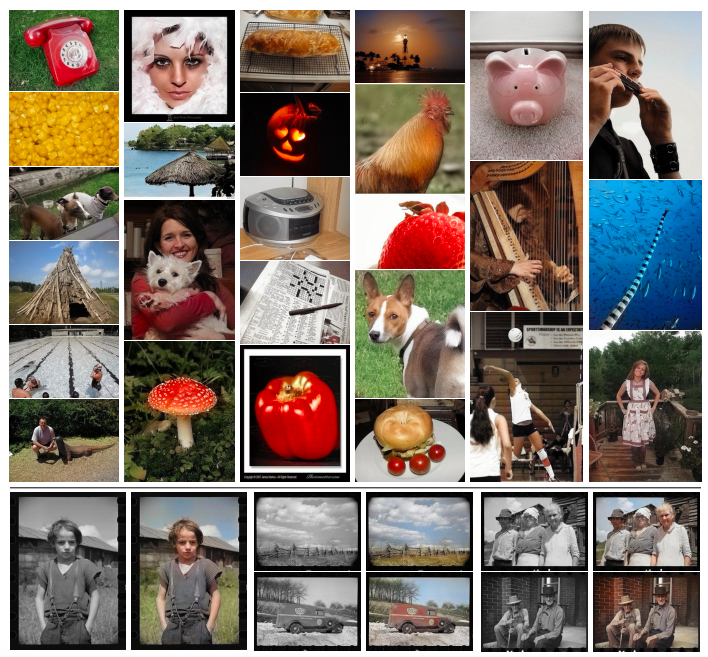
\includegraphics[width = 5in]{../images/LearnRepColorb}}

\slidetwo{Learning Representations for Colorization}{Larsson et al., March 2016}

\centerline{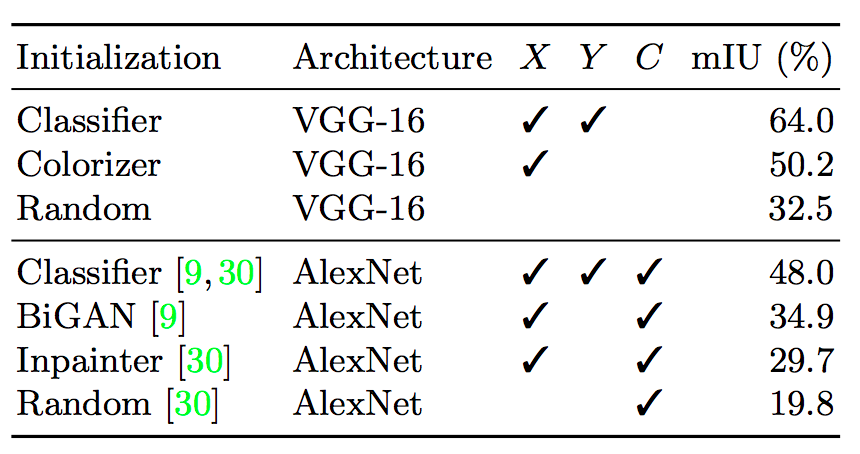
\includegraphics[width = 5in]{../images/LearnRepColorc}}
VGG-16, Pretrained on ImageNet evaluated on the PASCAL segmentation task.
Images Counts: {\color{red} Instagram 3.5G, ImageNet 14M, Pascal 5.7k}.
$X$ --- pretraining used, $Y$ ---pretrained with Labels, $C$ --- trained on PASCAL with color.

\slidetwo{Adding a Discrimination Loss}{to a Noisy-Channel RDA}

{\color{red} $$P_\Phi(y,z) = \pop(y)P_\Phi(z|y)$$}

\begin{eqnarray*}
\Phi^* & =  & \argmin_\Phi \left\{\begin{array}{l} I(y,z) \\
+ \lambda_1\;E_{y,z}\;\mathrm{Dist}(y,\hat{y}_\Phi(z)) \\
+ \lambda_2 \;E_{y,z}\;\mathrm{Discr}(y,\hat{y}_\Phi(z))\end{array}\right.
\end{eqnarray*}

\vfill
This can be viewed as an RDA with a discrimination distortion, or as a GAN with a rate-distortion objective.

\slidetwo{Adding a Discrimination Loss}{to a Conditional Noisy-Channel RDA}


\vfill
To model a class-conditional image distribution we might use the following where $x$ is a class label and $y$ is an image.

{\color{red} $$P_\Phi(x,y,z) = \pop(x,y)P_\Phi(z|y,x)$$}

\begin{eqnarray*}
\Phi^* & =  & \argmin_\Phi E_{x,y,z}\;\;\left\{\begin{array}{l} KL(P_\Phi(z|y,x),P_\Phi(z|x)) \\
+ \lambda_1\mathrm{Dist}(y,\;\hat{y}_\Phi(z)) \\
+ \lambda_2 \mathrm{Discr}(y,\;\hat{y}_\Phi(z)\;|\;x)\end{array}\right.
\end{eqnarray*}


\slidetwo{Contrastive Predictive Coding (CPC)}{van den Oord et al., July 2018}

\centerline{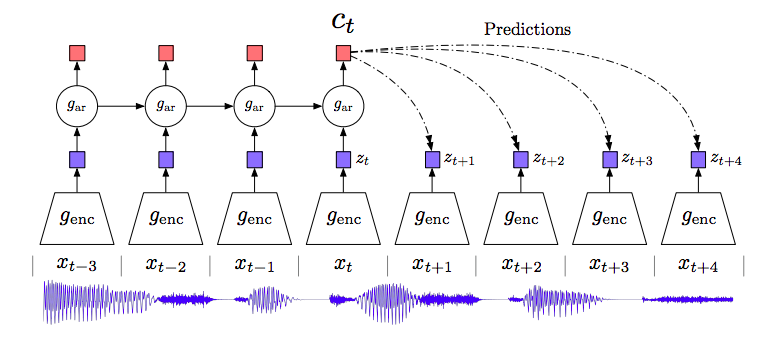
\includegraphics[height=3.5 in]{../images/MMI-PC}}

We $x_1$, $\ldots$ $x_t$ and make predictions about $x_{t+1}$, $\ldots$, $x_{t+k}$

\slidetwo{Contrastive Predictive Coding (CPC)}{van den Oord et al., July 2018}

\centerline{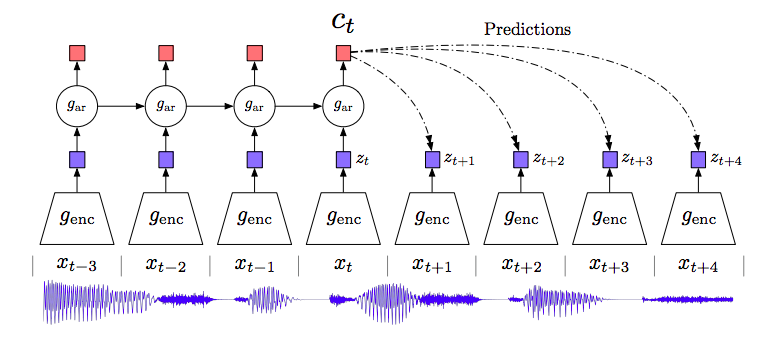
\includegraphics[height = 2.0in]{../images/MMI-PC}}

Rather than predict $x_{t+ \Delta t}$ we predict a feature vector $z_\Phi(x_t + \Delta t)$ from the feature vectors $z_\Phi(x_1)$, $\ldots$ $z_\Phi(x_t)$.

\vfill
We want the feature vector $z_\Phi(x)$ to carry the ``signal'' and drop the ``noise'' --- more later.

\slide{CPC}

\begin{eqnarray*}
\Phi^* & = & \argmin_\Phi\;\;E_{x_1,\ldots,x_t,\ldots,x_{t+k}} \;\sum_{\Delta t} \;\lambda_{\Delta t}\; {\cal L}_\mathrm{CEN}(x_{t+\Delta t}) \\
\\
{\cal L}_{\mathrm{CEN}}(x_{t+\Delta t}) & = & E_{x_1,\ldots x_N \sim \pop^N}\\
\\
& & \;\;\;-\ln P_\Phi(i|c_t,\Delta t,z_\Phi(x_{t+\Delta t}) \hookrightarrow z_\Phi(x_1),\ldots,z_\Phi(x_N))
\end{eqnarray*}

$$P_\Phi(i|c_t,\Delta t,z_1,\ldots,z_{N+1}) = {\color{red} \softmax_i\;z_iW_{\Delta t}\;c_t}$$

\vfill
The context $c_t$ and learned features $z_t$ must have {\color{red} linearly-extractable} information.

\slide{Maximizing a Lower Bound on Mutual Information}

\centerline{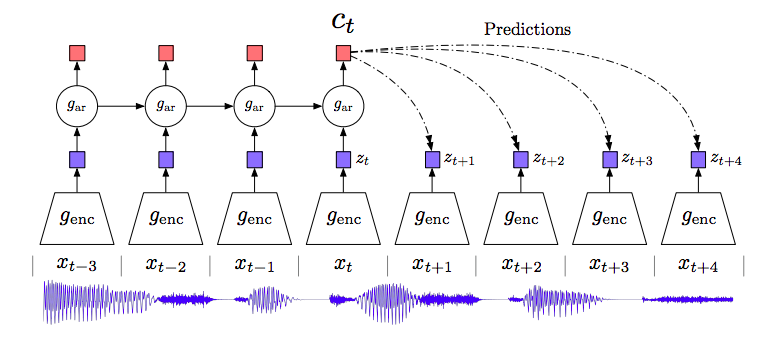
\includegraphics[height = 3.0in]{../images/MMI-PC}}

\begin{eqnarray*}
{\color{red} I(c_t,x_{t+\Delta t})} & {\color{red} \geq} & {\color{red} \ln (N +1) - {\cal L}_\mathrm{CEN}(\Delta t)}
\end{eqnarray*}

\vfill
By maximizing mutual information we are intuitively separating signal from noise.

\slide{CPC for Vision}

\centerline{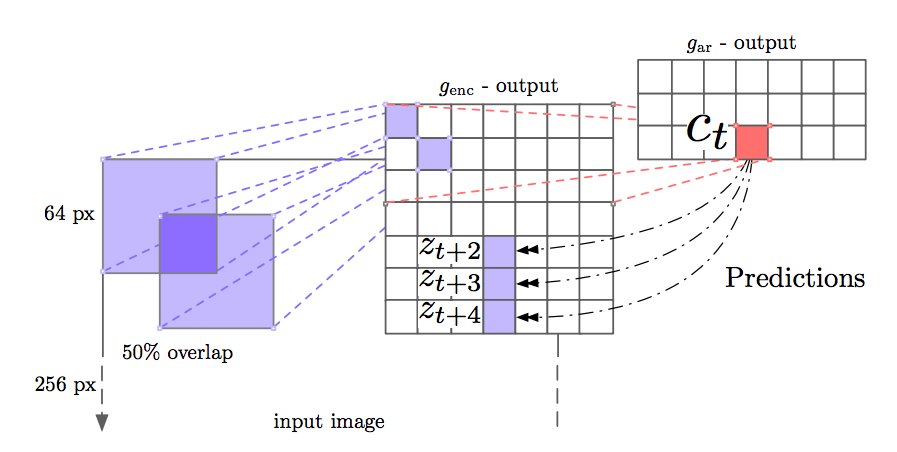
\includegraphics[width=8.0 in]{../images/LearnRepCTCb}}

\slide{CPC Vision Results}

\centerline{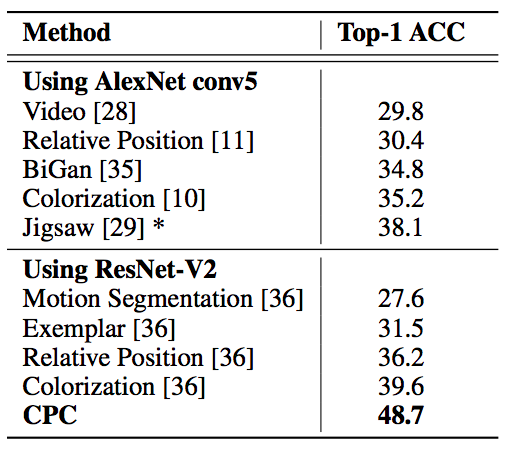
\includegraphics[height=3.5 in]{../images/LearnRepCTCc}}

Train and test are both on Imagenet but labels are only used retraining the final linear layer.

\vfill
Results are also give for speech recognition tasks and NLP tasks.


\slidetwo{Information Theoretic Co-Training}
{McAllester, Feb. 2018}

\centerline{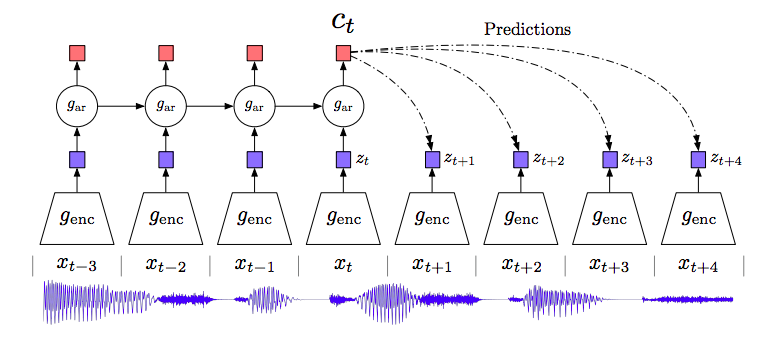
\includegraphics[height=2.25in]{../images/MMI-PC}}

$$\Phi^* = \argmax_\Phi\;\left(\sum_{\Delta t} \;\lambda_{\Delta t}\; \hat{I}(c,z_\Phi(x_{t+\Delta t}))\right) - \lambda \hat{H}(z_\Phi(x))$$

\vfill
$$\hat{I}(c,z_\Phi(x_{t+ \Delta t})) = \hat{H}(z_\Phi(x)) - \hat{H}(z_\Phi(x_{t+\Delta t})|c)$$

\slide{Difference of Entropy Models}

$$\hat{I}(c,z_\Phi(x_{t+ \Delta t})) = \hat{H}(z_\Phi(x)) - \hat{H}(z_\Phi(x_{t+\Delta t})|c)$$

We maximize the mutual information estimate where the entropy estimates are done with cross-entropy models --- upper bounds on true entropy.

\vfill
Note that maximizing $\hat{H}(z_\Phi(x))$ is adversarial --- $\Phi$ wants to increase the cross entropy while the cross entropy model
is trying to minimize the cross entropy.

\slide{Pretraining for NLP}

\begin{itemize}
\item Word Embeddings

\vfill
\item The Transformer

\vfill
\item ELMO, BERT and GPT-2
\end{itemize}

\slidetwo{Advances in Pre-Training Distributed Word Representations}
{Mikolov et al., 2017}

We want a mapping from a word $w$ to a vector $e(w)$ --- a word embedding.

\vfill
We can also consider phrase embedings $e(P)$ for a word sequence $P$.

\vfill
{\color{red} fastText} from Facebook is currently popular.

\vfill
It provides both contextual bag of words (cbow) and byte pair encoding (BPE) word vectors.

\slide{cbow word vectors}

We construct a population distribution on pairs $(c,w)$ here $c$ is a bag of word context and $w$ is a word.

\vfill
$$\Phi^* = \argmin_\Phi E_{c,w}\;-\ln P(w|c)$$

\vfill
$\Phi$ consists of a matrix $e[w,i]$ where $e[w,I]$ is the word embedding of $w$, and a matrix $e'[w,i]$ giving the embedding of the word
$w$ when it appears in a context.

\vfill
A score $s(w|c)$ is defined by
$$s(w|c) = \frac{1}{|c|} \sum_{w' \in c}\;e(w)^\top e'(w')$$

\slide{Negative Sampling in cbow}

\vfill
Rather than define $P_\Phi(w|c)$ by a softmax over $w$, one uses restricted negative sampling.

\vfill
We construct a training set of triples $(w,c,N_C)$

\vfill
$$\Phi^* = \argmin_\Phi\;E_{w,c,N_c}\;\ln\left(1 + e^{-s(w,c)}\right) + \sum_{n \in N_C} \ln\;\left(1 + e^{s(n,c)}\right)$$

\slide{Byte Pair Encoding (BPE)}

BPE constructs a set of character n-grams by starting with the unigrams and then greedily merging most common bigrams of n-grams.

\vfill
Given a set of character n-grams each word is treated as a bag of character n-grams.

\vfill
$$e[w] = \frac{1}{N} \sum_{n \in w}\; e(n)$$

\slidetwo{Attention is All You Need (the Transformer)}{Vaswani et al., June 2017}

The Transformer is based on multi-headed self-attention.

\centerline{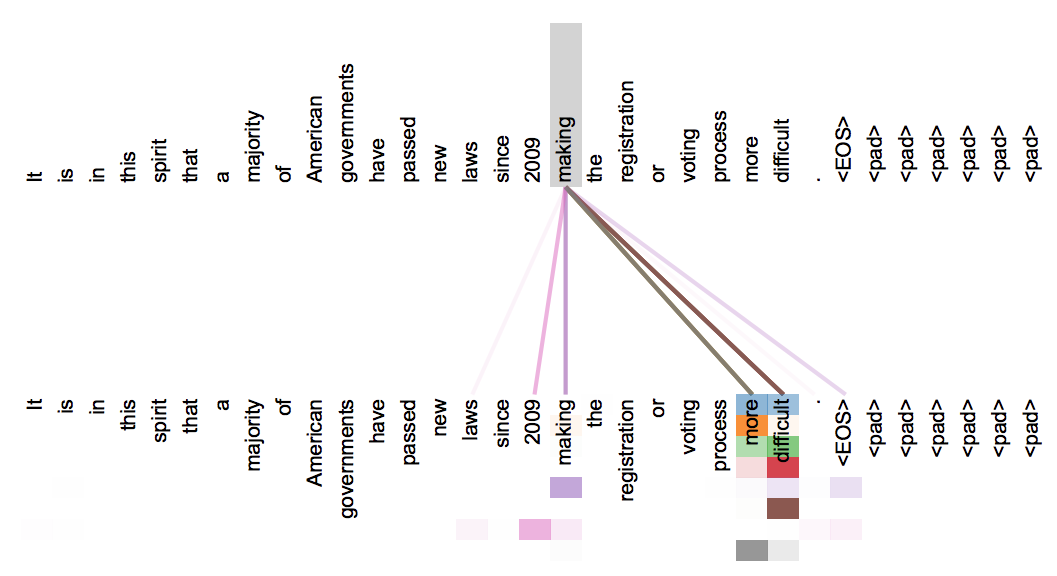
\includegraphics[height  = 3.5in]{../images/Transformera}}

\slide{Review of Attention}
Procedure $\mathrm{Lookup}(\mathrm{key}[J],\;M[T,J])$

\bigskip
\begin{eqnarray*}
s[t] & = &\mathrm{key}[J]^\top M[t,J] \\
\\
{\color{red} \alpha[t]} & {\color{red} =} & {\color{red} \softmax_t \;s[t]\;\mbox{; the attention}} \\
\\
{\color{red} V[J]} & {\color{red} =} & {\color{red} \sum_t\;\alpha[t]M[t,J]}
\end{eqnarray*}

\bigskip
Return $V[J]$

\slide{Multi-Layer, Multi-Headed Attention}

\vfill
Let $\ell$ ranger over layers --- each layer will be computed from the previous layer.

\vfill
Let $h$ range over ``heads'' --- each head is computing an attention for a different purpose.

\vfill
We will construct a layers of sequences of vectors $M[L,T,J]$.

\slide{Multi-Headed Self Attention}

To compute {\color{red} $M[\ell+1,T,J]$} from {\color{red} $M[\ell,T,J]$} we first compute:
      
\begin{eqnarray*}
\mathrm{Query}[\ell,h,t,{\color{red} k}] & = & \sum_j\;{\color{red} W^Q}[\ell,h,{\color{red} k,j}]M[\ell,t,{\color{red} j}] \\
\\
\mathrm{Key}[\ell,h,t,{\color{red} k}] & = & \sum_j\;{\color{red} W^K}[\ell,h,{\color{red} k,j}]M[\ell,t,{\color{red} j}] \\
\\
\mathrm{Value}[\ell,h,t,{\color{red} i}] & = & \sum_j\;{\color{red} W^V}[\ell,h,{\color{red} i,j}]M[\ell,t,{\color{red} j}]
\end{eqnarray*}

\slide{Multi-Headed Self Attention}

We then compute {\color{red} $M[\ell+1,T,J]$} as follows.

{\color{red}
\begin{eqnarray*}
s[\ell,h,t,t'] & = &\frac{1}{\sqrt{K}} \sum_k\;\mathrm{Query}[\ell,h,t,k]\mathrm{Key}[\ell,h,t',k] \\
\\
{\color{red} \alpha[\ell,h,t,t']} & {\color{red} =} & {\color{red} \softmax_{t'} \;s[\ell,h,t,t']}\;\;\;\mbox{the attention} \\
\\
V[\ell,h,t,i] & = & \sum_{t'}\;\alpha[\ell,h,t,t']\mathrm{Value}[\ell,h,t',i]
\end{eqnarray*}
}

{\color{red} $$M[\ell+1,t,J] = V[\ell,1,t,I];V[\ell,2,t,I];\cdots;V[\ell,H,t,I] \;\;\;\; J = HI$$}

\slide{Encoding Positional Information}

At the input layer we augment the word embeddings with position information. For example:

\vfill
{\color{red} $$M[0,t,J] = e[w[t],I];e^{i\omega t}\;;e^{i2\omega t}\;;e^{i4\omega t}\cdots;e^{i2^k\omega t}$$}

\vfill
This is analogous to adding a $k$-bit binary representation of $t$.

\vfill
Each complex number can be interpreted as a pointer on a dial.

\vfill
Each dial rotates twice as fast as the dial before.

\slide{The Transformer as a Translation Model}

\centerline{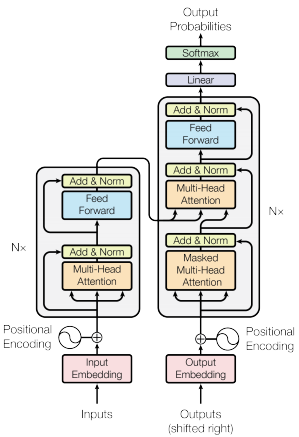
\includegraphics[height=5in]{../images/Transformerb}}




\slidetwo{Deep Contextualized Word Representations (ELMo)}{Peters et al., Feb. 2018 (AI2)}

\centerline{
\includegraphics[height = 1in]{../images/ELMob}}

\vfill
ELMo (EMbeddings from Language models) is a two layer bidirectional LSTM character language model trained to predict the next word
in both the forward and backward direction.

\vfill
It is designed to be used to generate ``contextual word embeddings'' as inputs to any system that uses word embeddings.

\slidetwo{Deep Contextualized Word Representations (ELMo)}{Peters et al., Feb. 2018 (AI2)}

\centerline{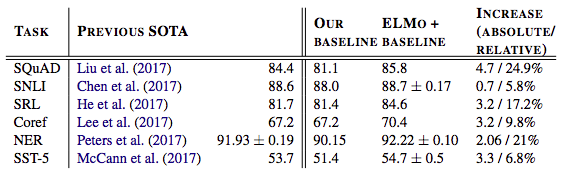
\includegraphics[width=8in]{../images/ELMo}}



\slidetwo{BERT: Pre-training of Deep Bidirectional Transformers}{Devlin et al., Oct. 2018 (Google AI Language)}

\centerline{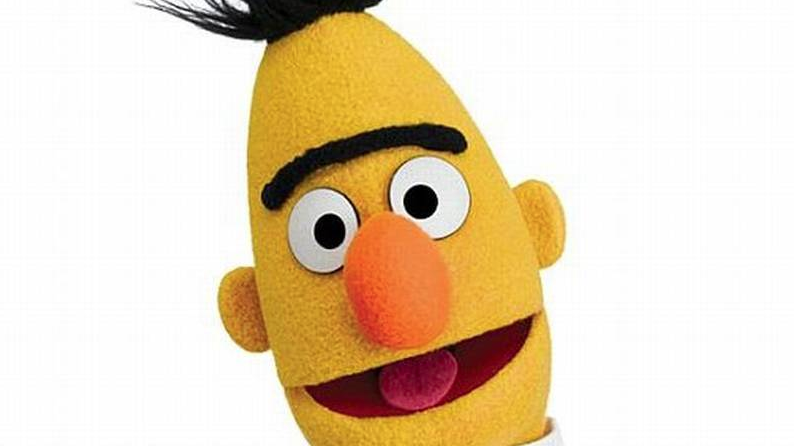
\includegraphics[height = 1in]{../images/BERTb}}

\vfill
BERT (Bidirectional Encoder Representations from Transformers) is Transformer language models trained to fill in sparse blanks that have been placed in text.

\vfill
It also generates sentence embeddings and has a second ``skip thought'' training criterion where it predicts the next senentence embedding (thought vector)
from the previous one.

\vfill It is designed to be used by adding a single task specific output layer and then fine tuning the entire model to the task.

\slidetwo{BERT: Pre-training of Deep Bidirectional Transformers}{Devlin et al., Oct. 2018 (Google AI Language)}

\centerline{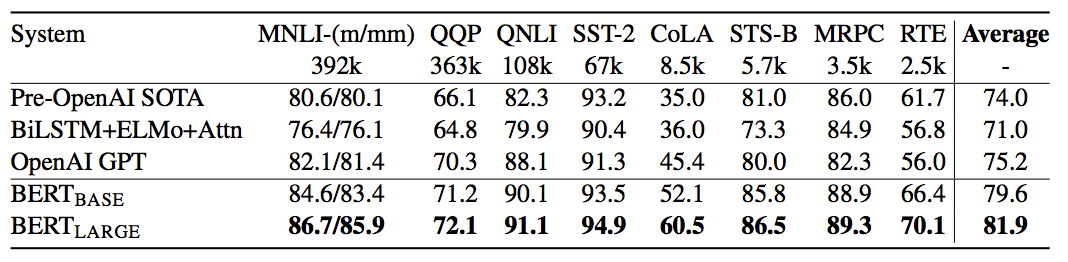
\includegraphics[width = 9in]{../images/BERTa}}

BERT results on the GLUE benchmark problems (General Language Understanding Evaluation) excluding the Winograd problems.
The first problem (MNLI -- Multi genre Natual Langauge Inference) has two metrics.  The number below each problem is the training set size.

\slide{GLUE tasks}

{\bf Sentiment Analysis} Given a sentence does it express positive or negative sentiment (toward a product in a product review). {\color{red} SST-2}.

\vfill
{\bf Natural Langauge Inference (NLI).}
Given a pair of sentences classify the relationship into ``entailed'', ``contradictory'' or ``netural''. {\color{red} MNLI, QNLI, RTE}.

\vfill
{\bf Semantic Equivalence.} Given two sentences do they express the same meaning. {\color{red} QQP, STS-B, MRPC}.

\vfill
{\bf Grammaticality Judgements.} Given a sentence is it grammatical. {\color{red} CoLA}.

\vfill
{\bf Winograd Problems.} Determine the referent of a pronoun in cases requiring semantics. {\color{red} WNLI}

\slidetwo{Language Models [are] Multitask Learners, (GPT-2)}{Radford et al., Feb. 2019 (Open AI)}

This is a Transformer language model trained on a new text corpus, webText, scraped from the internet and containing 40G words of text.

\vfill
Historically sampling text from a language model has yielded semantic gibberish.  This time things are different.

\vfill
\slide{Continuing from a Prompt}

{\color{red} Continue from:}

\vfill
In a shocking finding, scientist discovered a herd of unicorns living in a remote, previously unexplored valley, in the Andes Mountains. Even more surprising to the researchers was the fact that the unicorns spoke perfect English.

\slide{The Predicted Continuation}

{\color{red} Continuation excerpted from a single response, the response selected from 10 tries.}

\bigskip

The scientist named the population, after their distinctive horn, Ovid’s Unicorn. These four-horned, silver-white unicorns were previously unknown to science.

Now, after almost two centuries, the mystery of what sparked this odd phenomenon is finally solved.

Dr. Jorge Pérez, an evolutionary biologist from the University of La Paz, and several companions, were exploring the Andes Mountains when ...
Pérez and his friends were astonished to see the unicorn herd. ...
While examining these bizarre creatures the scientists discovered that the creatures also spoke some fairly regular English. Pérez stated, “We can see, for example, that they have a common ‘language,’ something like a dialect or dialectic.”

Dr. Pérez believes that the unicorns may have originated in Argentina ... some believe that perhaps the creatures were created when a human and a unicorn met each other in a time before human civilization. ... However, Pérez also pointed out that it is likely that the only way of knowing for sure if unicorns are indeed the descendants of a lost alien race is through DNA. ...

\slide{A Laguage Model Translating French to English}

{\color{red} Continue from: $<$French1$>$ = $<$English1$>$, ... ,$<$Frenchn$>$ = $<$Englishn$>$, $<$French$>$ =}

\vfill
Note that the translation pairs in the prompt do not influence the model parameters.

\vfill
\centerline{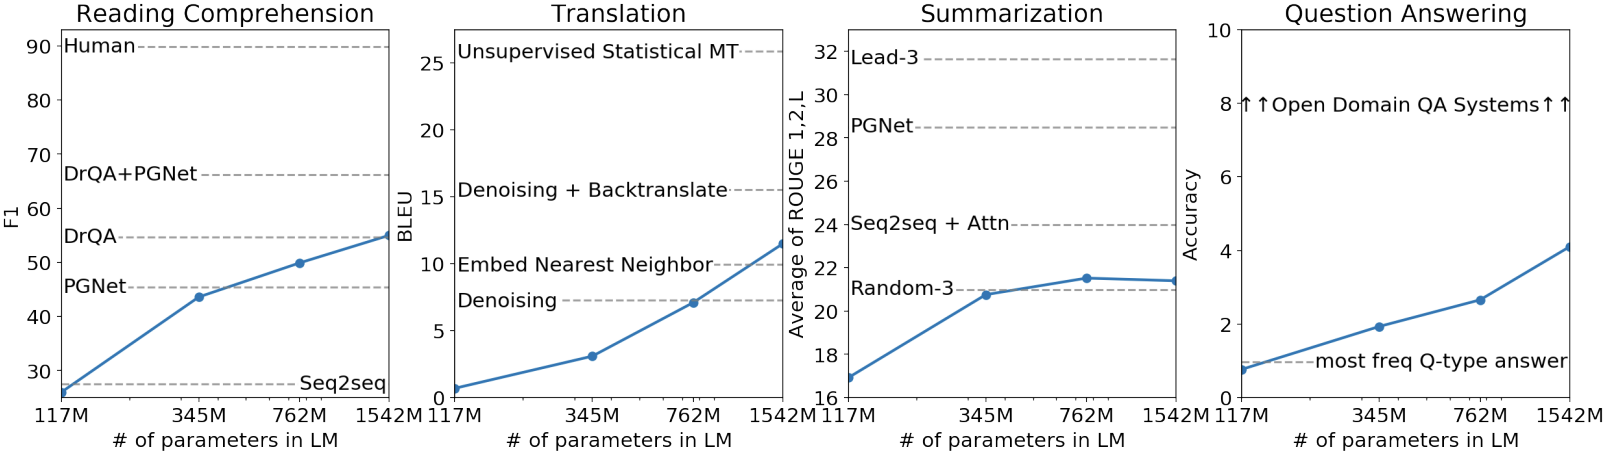
\includegraphics[width = 9in]{../images/GPT-2a}}


\slide{END}

}
\end{document}
